\documentclass[a5paper,pagesize,french]{book}

\usepackage{babel}

\pagestyle{empty}

%% better use this ('usepackage') for a5paper !!
\usepackage[top=0.25cm, bottom=0.25cm, left=0.25cm, right=0.25cm]{geometry}
% gauche, haut, droite, bas, entete, ente2txt, pied, txt2pied
% \usepackage{vmargin}
% \setmarginsrb{0.25cm}{0.25cm}{0.25cm}{0.25cm}{0pt}{0pt}{0pt}{0pt}

\usepackage{mathtools}
\usepackage{fontspec} %% fontes / polices de caracteres

% \usepackage{xkeyval}		% Load xkeyval first ??
% \usepackage{JeuxCartes}	%% dépendance vers defKV dans simplekv, version 2021++
% \usepackage{babel}

% \defaultfontfeatures{Mapping=tex-text,Scale=MatchLowercase}
\setmainfont{Liberation Serif} 

%% \usepackage{fdsymbol} %% commented because conflict with packages 'fontspec' / 'JeuxCartes'
%% \clubsuit
%% \vardiamondsuit
%% \spadesuit
%% \varheartsuit
\DeclareSymbolFont{extraup}{U}{zavm}{m}{n}
\DeclareMathSymbol{\varheart}{\mathalpha}{extraup}{86}
\DeclareMathSymbol{\vardiamond}{\mathalpha}{extraup}{87}

\usepackage{fancybox} %% boxes

\usepackage{tikz}

\begin{document}

\setlength\parindent{0pt} % \noindent for all document

% $\heartsuit \varheart \diamondsuit \vardiamond \clubsuit \spadesuit$ ~\\

% {\color{red} $\heartsuit$ }
% {\color{red} $\diamondsuit$ }

% {\color{red} $\varheart$ }
% {\color{red} $\vardiamond$ }

%% {\centering \Huge{Château FalkenStein} }~\\
%% {\centering \large{Journal Intime} }~\\

\begin{center}
	\begin{tabular}[c]{ p{0.20\textwidth} p{0.45\textwidth} p{0.20\textwidth} }
		
\includegraphics[width=0.20\textwidth]{../../images/artsdecos/ornement01whiteBG.png} & 
			\centering
			{ \Huge{\setmainfont{Chomsky} Château FalkenStein } }~\newline~\newline~\newline
			{ \LARGE{ \setmainfont{Z003} Journal Intime } }
			{ \Large{ \setmainfont{Z003} Description Partie 1 sur 2} }
		& 
\includegraphics[width=0.20\textwidth]{../../images/artsdecos/ornement01whiteBG.png} \\
	\end{tabular}
\end{center}

\begin{tabular}[c]{ p{0.45\textwidth} p{0.45\textwidth} }
	NOM						&									\\
	ORIGINE					&		RÉSIDENCE					\\
	APPARENCE PHYSIQUE		&									\\
							&									\\
							&									\\
							&									\\
	ENFANCE / ÉDUCATION		&									\\
							&									\\
							&									\\
							&									\\
	GRANDES QUALITÉS		&		PIRES DÉFAUTS				\\
							&									\\
							&									\\
							&									\\
	STYLE					&									\\
							&									\\
							&									\\
							&									\\
	PERSONNALITÉ			&									\\
							&									\\
							&									\\
							&									\\
	CHOSES LES PLUS AIMÉES	&		CHOSES LES PLUS DÉTESTÉES	\\
							&									\\
							&									\\
							&									\\
\end{tabular}

\clearpage

\begin{center}
	\begin{tabular}[c]{ p{0.20\textwidth} p{0.45\textwidth} p{0.20\textwidth} }
		
\includegraphics[width=0.20\textwidth]{../../images/artsdecos/ornement04whiteBG.png} & 
			\centering
			{ \Huge{\setmainfont{Chomsky} Château FalkenStein } }~\newline~\newline~\newline
			{ \LARGE{ \setmainfont{Z003} Journal Intime } }
			{ \Large{ \setmainfont{Z003} Description Partie 2 sur 2} }
		& 
\includegraphics[width=0.20\textwidth]{../../images/artsdecos/ornement04whiteBG.png} \\
	\end{tabular}
\end{center}

\begin{tabular}[c]{ p{0.45\textwidth} p{0.45\textwidth} }
	PRINCIPES				&									\\
							&									\\
	BIEN LE PLUS PRÉCIEUX	&									\\
							&									\\
	PERSONNE LA PLUS AIMÉE	&									\\
							&									\\
	ENNEMI JURÉ				&		ALLIÉS						\\
							&									\\
							&									\\
							&									\\
	VIE ROMANTIQUE			&									\\
							&									\\
	BUT SOCIAL				&									\\
							&									\\
	BUT PROFESSIONNEL		&									\\
							&									\\
	BUT AMOUREUX			&									\\
							&									\\
	PLUS GRAND REGRET		&		PLUS GRANDE FIERTÉ			\\
							&									\\
							&									\\
							&									\\
	HISTOIRE RÉCENTE		&									\\
							&									\\
							&									\\
							&									\\
\end{tabular}

\clearpage

\begin{center}
	\begin{tabular}[c]{ p{0.20\textwidth} p{0.45\textwidth} p{0.20\textwidth} }
		
\includegraphics[width=0.20\textwidth]{../../images/artsdecos/ornement03whiteBG.png} & 
			\centering
			{ \Huge{\setmainfont{Chomsky} Château FalkenStein } }~\newline~\newline~\newline
			{ \LARGE{ \setmainfont{Z003} Memento \& Usages } }
		& 
\includegraphics[width=0.20\textwidth]{../../images/artsdecos/ornement03whiteBG.png} \\
	\end{tabular}
\end{center}

\begin{minipage}[ht]{0.95\textwidth}
	Niveau des Talents : FAIble ; MOYen ; BON ; EXCellent ; MAGistral ; PROdigieux~\newline~\newline
	Par défaut un Talent est MOYen ; à la création un personnage dispose de : 
	\begin{itemize}
		\item un Talent EXCellent, 
		\item un Talent FAIble et, 
		\item quatre Talents BON. 
	\end{itemize}~\\
	Pour tous talent supplémentaire EXCellent, choisir un Talent FAIble.~\newline
	Pour tous talent supplémentaire MAGistral, choisir deux Talents FAIble.~\newline
	Pour tous talent supplémentaire PROdigieux, choisir trois Talents FAIble.~\newline~\newline
	Lors d'une épreuve, toute carte de la bonne couleur a sa valeur faciale : du 2 à 10, plus Valet (11), Dame (12), Roi (13), As (14), un Joker vaut 15, tout autre carte vaut 1 !
\end{minipage}~\\~\\

%% DONE memo des tirages possibles

\begin{center}
	\begin{tabular}[c]{ c c c c c }
		
\includegraphics[width=0.15\textwidth]{../../images/artsdecos/ornement01whiteBG.png}	&	
		
\includegraphics[width=0.15\textwidth]{../../images/artsdecos/ornement02whiteBG.png}	&	
		
\includegraphics[width=0.15\textwidth]{../../images/artsdecos/ornement03whiteBG.png}	&	
		
\includegraphics[width=0.15\textwidth]{../../images/artsdecos/ornement04whiteBG.png}	&	
		
\includegraphics[width=0.15\textwidth]{../../images/artsdecos/ornement05whiteBG.png}	\\
		
\includegraphics[width=0.15\textwidth]{../../images/artsdecos/ornement06whiteBG.png}	&	
		
\includegraphics[width=0.15\textwidth]{../../images/artsdecos/ornement07whiteBG.png}	&	
		
\includegraphics[width=0.15\textwidth]{../../images/artsdecos/ornement08whiteBG.png}	&	
		
\includegraphics[width=0.15\textwidth]{../../images/artsdecos/ornement09whiteBG.png}	&	
		
\includegraphics[width=0.15\textwidth]{../../images/artsdecos/ornement10whiteBG.png}	\\
	\end{tabular}
\end{center}

\begin{center}
	{ \setmainfont{Z003} Merci de favoriser le Jeu Du Rôle (<<RolePlay>>) et restez digne en toutes circonstances ! }
\end{center}~\\

%% TODO utilisation de JeuxCartes

\begin{center}
	\begin{tabular}[c]{ c c c }

		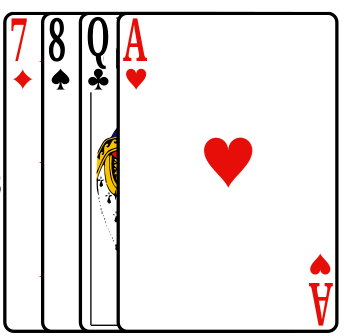
\includegraphics[width=0.20\textwidth]{img/MainCarteExample1.png} &	
		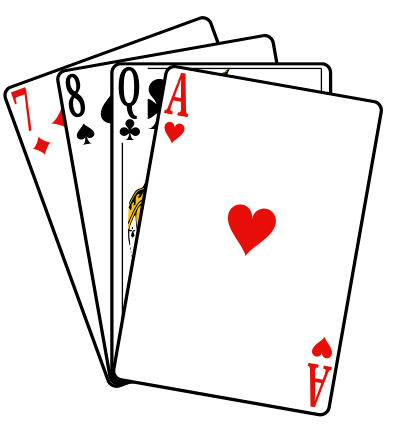
\includegraphics[width=0.20\textwidth]{img/MainCarteExample2.png} &	
		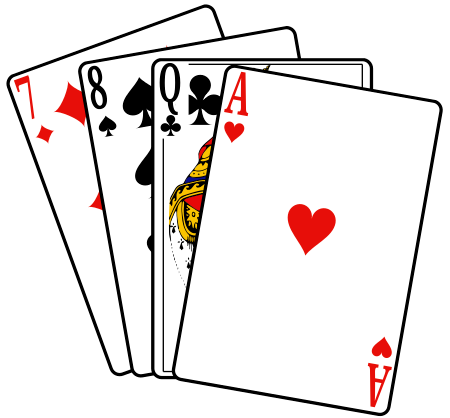
\includegraphics[width=0.20\textwidth]{img/MainCarteExample3.png} \\

	\end{tabular}
\end{center}

%% \MainCartesJeu{7K § 8P § DT § AC}
%% ~ou \MainCartesJeu[Eventail,EspH=0,EspV=0.1]{7K § 8P § DT § AC}
%% ~ou \MainCartesJeu[Eventail,EspH=0.5]{7K § 8P § DT § AC}

%% Ça c'est une belle poignée ! \MainCartesJeu[Inverse,Eventail,Hauteur=3,TypeJeu=Tarot,EspH=0,EspV=0.1]%
%% {Exc § 1AT § 2AT § 3AT § 4AT § 5AT § 6AT § %
%% 10AT § 11AT § 15AT § 16AT § 19AT § 20AT § 21AT}

%% \clearpage

\clearpage

%% {\centering \Huge{Château FalkenStein} }~\\
%% {\centering \large{Fiche Principale} }~\\

\begin{center}
	\begin{tabular}[c]{ p{0.20\textwidth} p{0.45\textwidth} p{0.20\textwidth} }
		
\includegraphics[width=0.20\textwidth]{../../images/artsdecos/ornement08whiteBG.png} & 
			\centering
			{ \Huge{\setmainfont{Chomsky} Château FalkenStein } }~\newline~\newline~\newline
			{ \LARGE{ \setmainfont{Z003} Fiche Principale (2 Pages) } }
		& 
\includegraphics[width=0.20\textwidth]{../../images/artsdecos/ornement08whiteBG.png} \\
	\end{tabular}
\end{center}

\begin{minipage}[ht]{0.48\textwidth}
	NOM~\newline
\end{minipage} \hfill \begin{minipage}[ht]{0.48\textwidth}
	ARCHÉTYPE~\newline
\end{minipage}~\\~\\

%% FAIble ; MOYen ; BON ; EXCellent ; EXcePtionnel ; EXTradordinaire
%% FAIble ; MOYen ; BON ; EXCellent ; MAGistral ; PROdigieux

\begin{tabular}[c]{|p{0.30\textwidth}|p{0.08\textwidth}|p{0.08\textwidth}|p{0.08\textwidth}|p{0.08\textwidth}|p{0.08\textwidth}|p{0.08\textwidth}|}
	\hline
	\textbf{TALENTS}									&	FAI (2)	&	MOY (4)	&	BON (6)	&	EXC (8)	&	MAG (10)	&	PRO (12)	\\ \hline
	AGILITÉ { $\clubsuit$ }								&	$\circ$	&	$\circ$	&	$\circ$	&	$\circ$	&	$\circ$		&	$\circ$		\\ \hline
	AISANCE SOCIALE { $\spadesuit$ }					&	$\circ$	&	$\circ$	&	$\circ$	&	$\circ$	&	$\circ$		&	$\circ$		\\ \hline
	ARTISANAT {\color{red} $\vardiamond$ }				&	$\circ$	&	$\circ$	&	$\circ$	&	$\circ$	&	$\circ$		&	$\circ$		\\ \hline	
	% ATTRACTION {\color{red} $\varheart$ }				&	$\circ$	&	$\circ$	&	$\circ$	&	$\circ$	&	$\circ$		&	$\circ$		\\ \hline
	BARREUR {\color{red} $\vardiamond$ }				&	$\circ$	&	$\circ$	&	$\circ$	&	$\circ$	&	$\circ$		&	$\circ$		\\ \hline
	BRICOLAGE {\color{red} $\vardiamond$ }				&	$\circ$	&	$\circ$	&	$\circ$	&	$\circ$	&	$\circ$		&	$\circ$		\\ \hline
	CHARISME {\color{red} $\varheart$ }					&	$\circ$	&	$\circ$	&	$\circ$	&	$\circ$	&	$\circ$		&	$\circ$		\\ \hline
	CHARME ( FAË ) {\color{red} $\varheart$ }			&	$\circ$	&	$\circ$	&	$\circ$	&	$\circ$	&	$\circ$		&	$\circ$		\\ \hline
	COMMANDEMENT {\color{red} $\varheart$ }				&	$\circ$	&	$\circ$	&	$\circ$	&	$\circ$	&	$\circ$		&	$\circ$		\\ \hline
	COMMERCE {\color{red} $\varheart$ }					&	$\circ$	&	$\circ$	&	$\circ$	&	$\circ$	&	$\circ$		&	$\circ$		\\ \hline
	CONDUITE { $\clubsuit$ }							&	$\circ$	&	$\circ$	&	$\circ$	&	$\circ$	&	$\circ$		&	$\circ$		\\ \hline
	COURAGE {\color{red} $\varheart$ }					&	$\circ$	&	$\circ$	&	$\circ$	&	$\circ$	&	$\circ$		&	$\circ$		\\ \hline
	DISCRÉTION { $\clubsuit$ }							&	$\circ$	&	$\circ$	&	$\circ$	&	$\circ$	&	$\circ$		&	$\circ$		\\ \hline
	% ÉLEVAGE {\color{red} $\varheart$ }					&	$\circ$	&	$\circ$	&	$\circ$	&	$\circ$	&	$\circ$		&	$\circ$		\\ \hline
	ÉQUITATION { $\clubsuit$ }							&	$\circ$	&	$\circ$	&	$\circ$	&	$\circ$	&	$\circ$		&	$\circ$		\\ \hline
	ESCRIME { $\clubsuit$ }								&	$\circ$	&	$\circ$	&	$\circ$	&	$\circ$	&	$\circ$		&	$\circ$		\\ \hline
	ÉTHÉRALITÉ ( FAË ) { $\clubsuit$ }					&	$\circ$	&	$\circ$	&	$\circ$	&	$\circ$	&	$\circ$		&	$\circ$		\\ \hline
	FINANCES { $\spadesuit$ }							&	$\circ$	&	$\circ$	&	$\circ$	&	$\circ$	&	$\circ$		&	$\circ$		\\ \hline
	INGÉNIERIE MAGIQUE {\color{red} $\vardiamond$ }		&	$\circ$	&	$\circ$	&	$\circ$	&	$\circ$	&	$\circ$		&	$\circ$		\\ \hline
	INSTRUCTION {\color{red} $\vardiamond$ }			&	$\circ$	&	$\circ$	&	$\circ$	&	$\circ$	&	$\circ$		&	$\circ$		\\ \hline
	INTERPRÉTATION {\color{red} $\varheart$ }			&	$\circ$	&	$\circ$	&	$\circ$	&	$\circ$	&	$\circ$		&	$\circ$		\\ \hline
	INVENTION {\color{red} $\vardiamond$ }				&	$\circ$	&	$\circ$	&	$\circ$	&	$\circ$	&	$\circ$		&	$\circ$		\\ \hline
	JEU {\color{red} $\vardiamond$ }					&	$\circ$	&	$\circ$	&	$\circ$	&	$\circ$	&	$\circ$		&	$\circ$		\\ \hline
	MÉDECINE {\color{red} $\vardiamond$ }				&	$\circ$	&	$\circ$	&	$\circ$	&	$\circ$	&	$\circ$		&	$\circ$		\\ \hline
	% MÊLÉE { $\clubsuit$ }								&	$\circ$	&	$\circ$	&	$\circ$	&	$\circ$	&	$\circ$		&	$\circ$		\\ \hline
	MÉTAMORPHOSE ( FAË ) { $\clubsuit$ }				&	$\circ$	&	$\circ$	&	$\circ$	&	$\circ$	&	$\circ$		&	$\circ$		\\ \hline
	MESMÉRISME {\color{red} $\varheart$ }				&	$\circ$	&	$\circ$	&	$\circ$	&	$\circ$	&	$\circ$		&	$\circ$		\\ \hline
	PERCEPTION {\color{red} $\vardiamond$ }				&	$\circ$	&	$\circ$	&	$\circ$	&	$\circ$	&	$\circ$		&	$\circ$		\\ \hline
	PHYSIQUE { $\clubsuit$ }							&	$\circ$	&	$\circ$	&	$\circ$	&	$\circ$	&	$\circ$		&	$\circ$		\\ \hline
	PUGILAT { $\clubsuit$ }								&	$\circ$	&	$\circ$	&	$\circ$	&	$\circ$	&	$\circ$		&	$\circ$		\\ \hline
	POUVOIR FAË {\color{red} $\vardiamond$ }			&	$\circ$	&	$\circ$	&	$\circ$	&	$\circ$	&	$\circ$		&	$\circ$		\\ \hline
	RELATIONS { $\spadesuit$ }							&	$\circ$	&	$\circ$	&	$\circ$	&	$\circ$	&	$\circ$		&	$\circ$		\\ \hline
	% RENOM { $\spadesuit$ }								&	$\circ$	&	$\circ$	&	$\circ$	&	$\circ$	&	$\circ$		&	$\circ$		\\ \hline
	% SCIENCES NATURELLES {\color{red} $\vardiamond$ }	&	$\circ$	&	$\circ$	&	$\circ$	&	$\circ$	&	$\circ$		&	$\circ$		\\ \hline
	SORCELLERIE {\color{red} $\vardiamond$ }			&	$\circ$	&	$\circ$	&	$\circ$	&	$\circ$	&	$\circ$		&	$\circ$		\\ \hline
	TIR { $\clubsuit$ }									&	$\circ$	&	$\circ$	&	$\circ$	&	$\circ$	&	$\circ$		&	$\circ$		\\ \hline
\end{tabular}

\clearpage

\begin{minipage}[ht]{0.48\textwidth}
	\begin{tabular}[c]{|p{0.10\textwidth}|c|c|c|c|c|c|c|}
		%% \foreach \x in {-7,-6,...,10,11}	{ \x &	} 
		%% 12	\\
		\hline
		\textbf{Santé}	&	-7	&	-6	&	-5	&	-4	&	-3	&	-2	&	-1	\\ \hline
						&	0	&	1	&	2	&	3	&	4	&	5	&	6	\\ \hline
						&	7	&	8	&	9	&	10	&	11	&	12	&		\\ \hline
	\end{tabular}
\end{minipage} \hfill \begin{minipage}[ht]{0.48\textwidth}
	
\includegraphics[width=0.50\textwidth]{../../images/artsdecos/ornement06whiteBG.png}
\end{minipage}~\\~\\

\begin{tabular}[c]{|p{0.10\textwidth}|p{0.10\textwidth}|p{0.10\textwidth}|p{0.15\textwidth}|p{0.10\textwidth}|p{0.10\textwidth}|p{0.10\textwidth}|} 
	\hline
	\textbf{ARMES}	&	PORTÉE	&	MUN.	&	DISCRÉTION	&	BP	&	BT	&	BM	\\
	\hline
					&			&			&				&		&		&		\\
	\hline
					&			&			&				&		&		&		\\
	\hline
					&			&			&				&		&		&		\\
	\hline
\end{tabular}~\\~\\

\shadowbox{ \begin{minipage}[ht]{0.95\textwidth}
	\textbf{BIENS, SORTS ET NOTES}~\\~\\~\\~\\~\\
\end{minipage} }~\\~\\

%% \clearpage

	\shadowbox{ \begin{minipage}[ht]{0.95\textwidth}
			\textbf{Portrait}	~\newline~\newline~\newline~\newline~\newline~\newline~\newline~\newline
								~\newline~\newline~\newline~\newline~\newline~\newline~\newline~\newline
								~\newline~\newline~\newline~\newline~\newline~\newline~\newline~\newline
	\end{minipage} }~\\~\\

\clearpage

%% DONE répéter page pointillée !!
\foreach \pages in {1,2,...,58}{% DONE complétion à 64 PAGES !! (58 à priori)
	% \tikz \foreach \x / \y in {1/1,2/2...,30/20} \draw (\x,\y) circle (0.25);
	\begin{tikzpicture}
		\foreach \x in {0,0.5,...,14 } %% 15 | paperwidth | textwidth
			\foreach \y in {0,0.5,...,20 } %% 20 | paperheight | textheight
				{ \draw (\x,\y) circle (0.01); }
	\end{tikzpicture}
	\clearpage
}%

\clearpage

~\\ \dotfill~\\

\hfill

\emph{Château FalkenStein} est un Jeu de Rôle "sur table" (JdR / TTRPG en anglais) créé par \emph{Mike Ponsmith} (CyberPunk 2020, CyberPunk Red, CyberPunk 2077, Mekton Z...) en 1994, marque déposée par R.TalsorianGames.~\\
\emph{Château FalkenStein} re-édité en France par les éditions \emph{Lapin Marteau} en 2021.~\\

Le présent carnet conçu par \emph{Gabriel Chandesris} en 2025 pour les rôlistes de la \emph{Ligue Ludique} (Paris).~\\
\today~\\

Réalisé avec \LaTeX ; polices de caractères "Liberation Serif", {\setmainfont{Chomsky} Chomsky } et { \setmainfont{Z003} Z003 } ; package 'JeuxCartes' (et 'tikz', forcément). 
  
\end{document}
